\documentclass[a4paper, 12pt, british]{article}
\usepackage[british]{babel}
\usepackage{microtype}
\usepackage{graphicx}
\usepackage{caption}
\usepackage{wrapfig}
\usepackage{lscape}
\usepackage{rotating}
\usepackage{epstopdf}
\usepackage{enumitem}
\usepackage{natbib}
\usepackage[dvipsnames]{xcolor}
\usepackage[automake]{glossaries-extra}
\usepackage{longtable}
\usepackage{refstyle}
\usepackage[colorlinks=true,linkcolor=BrickRed,citecolor=Fuchsia]{hyperref}

\graphicspath{ {images/} }

\loadglsentries{glossary.tex}
\makeglossaries

\begin{document}

\date{\today}
\author{Callum John Spiller}

\title{%
    Spatialisation as a Service (SaaS) \\
    \large Project Definition }

\maketitle
\newpage
\tableofcontents
\newpage

\section{Project Aims}\label{sec:project-aims}
The primary aim of this project is to research, design, and implement a web service that allows a user to easily experience ambisonic audio based on their own inputs.\ Spatial audio is a paradigm that is emergent in modern entertainment systems;\ most prominently in the PlayStation 5 system that is designed and produced by \gls{sie}.

This project is based upon the hypothesis that, for a user who wishes to experiment with or experience ambisonic audio, the barrier for entry is too high.\ Engaging with a working demonstration of customisable ambisonic audio requires a user to perform a significant amount of preparation on a local machine;\ it demands a time commitment and pre-requisite technical knowledge that is far greater than is reasonable for an interested user to quickly evaluate what is possible.

This project aims to produce and test a working example of a stereo-to-ambisonic conversion tool that leverages the accessibility benefits of internet technology and cloud infrastructure.\ The imagined workflow would allow a user to use a standard web browser\footnote{The project will most likely be designed for interaction through Chromium-based browsers and Firefox} to upload an audio file to a website and then receive back a new audio file that has rendered the stems from the original file into a `spatialised' format that is informed by \glspl{hrtf}.\ All the audio processing will execute in \gls{aws} cloud environments.

\section{Project Objectives}\label{sec:project-objectives}

In order to achieve the aims set out in Section~\ref{sec:project-aims} the project must produce a number of deliverables:

\begin{enumerate}
    \item A project plan\footnote{Find an initial draft of this plan in Section ~\ref{sec:project-plan}. Note that this plan is subject to change as the project progresses.} which outlines the timeline of both the research and development of the project
    \item A review of pertinent literature relating primarily to:
    \begin{itemize}
        \item Audio spatialisation
        \item Web audio \glspl{api}
        \item Cloud infrastructure (including those available from \gls{aws})
    \end{itemize}
    \item A review of existing stereo-to-ambisonic services and technologies.
    \item A functioning stereo-to-ambisonic serverless pipeline.
    \item A frontend that enables a user to interact with the conversion pipeline by uploading and downloading audio files, as well as setting parameters for conversion through a web \gls{api}.
    \item A testing framework that supports iterative development.
    \item A report on user testing, including feedback from stakeholders.
    \item A review and analysis of how the produced system has met or missed the targets.
\end{enumerate}

These deliverables will be produced in addition to the artefacts required of the project timeline, namely:

\begin{enumerate}
    \item Interim report
    \item Progress presentation
    \item Draft report
    \item Project video
\end{enumerate}

The production of these subsidiary artefacts will ensure the constant monitoring of the project.\ Having this level of accountability as the project timeline progresses will ensure a constant tending to the project.

\subsection{Learning Outcome Mapping}\label{subsec:learning-outcome-mapping}

This project is executed as part of the BSc Digital \& Technology Solutions (Software Engineer) programme.\ This programme has a set of learning outcomes that comprise the programme specification.\ Find below a~\hyperref[tab:lo_mapping]{mapping} of the aspects of this project that correspond to these learning outcomes.



\begin{longtable}{| p{0.07\linewidth} | p{0.4\linewidth} | p{0.4\linewidth} |}
    \hline
    Code & Description & Mapping \\
    \hline
    \hline
    A1 & Understanding of business operations, procedures and culture applicable to a sustainable career as a Digital \& Technology Solutions professional.\ & This project will be undertaken using an iterative development methodology, similar to that used in professional development teams. \\
    \hline
    A2 & Critical understanding and analysis of the theoretical, conceptual and practical issues central to the practice of developing, implementing and maintaining technology solutions.\ & The execution of the project will highlight practical issues of software project implementation, while engaging the theoretical understanding of development issues gained as a part of the programme. \\
    \hline
    A3 & A real workplace learning pedagogy in order to develop the competences required by employers.\ & Given that, in the workplace, the realities of software development in a commercial environment become more apparent, this project will allow the implementation of the lessons learnt while undergoing the apprenticeship in addition to granting a greater amount of oversight on an individual project. \\
    \hline
    A4 & Knowledge of project, people, and resource management principles and techniques.\ & This project is self-sustained and requires engagement with stakeholders and project supervisors both at university and in the workplace. \\
    \hline
    \hline
    B1 & Demonstrate competence and independence in technology solutions to form a solid foundation for further
    development.\ & A project developed without other team-members is an exhibition of competence across the entire software development lifecycle as a single person will have to execute the entire project and not rely on others to do work for them. \\
    \hline
    B2 & Identify, select, apply, and evaluate advanced problem-solving and modelling skills appropriate to developing technology solutions for business.\ & As a part of the planning and implementation stages of the project, strong modelling and problem-solving skills should be demonstrated. \\
    \hline
    B3 & Demonstrate advanced practical skills in the chosen area of IT occupational competence.\ & This project requires a high level of knowledge in both audio processing and cloud development.\ If a working prototype is achieved, then this will demonstrate strong practical skills. \\
    \hline
    B4 & Appreciate the challenges associated with industry standard methodologies, processes, techniques and tools
    associated with the chosen area of IT occupational competence.\ & Engaging with the project will create exposure to the practical challenges associated with audio, web, and cloud development.\ Troubleshooting the project will be factored into development time.\\
    \hline
    \hline
    C1 & Able to engage effectively with staff all levels in the organisation.\ & Utilising contacts and resources at work will be crucial to the success of this project. \\
    \hline
    C2 & Motivated to learn from experience in a technology solutions project-oriented environment.\ & Engaging with the project will result in lessons learnt from experience. \\
    \hline
    C3 & Able to manage own personal and professional development.\ & To enact the project successfully, a high level of personal organisation is required.\ This project will be monitored and recorded using project-management software. \\
    \hline
    C4 & Able to display initiative and resilience in the face of new challenges.\ & Despite the fact that a large amount of planning and analysis will be performed as a part of the project, unforeseen challenges will force the re-assessment of the project in light of them. \\
    \hline

    \caption{Learning outcome mapping}
    \label{tab:lo_mapping}
\end{longtable}

\subsection{Business Area Mapping}\label{subsec:business-area-mapping}
This project is being undertaken as a part of a degree apprenticeship that is being sponsored by~\gls{sie}.\ Spatial audio is an area of particular significance to the company given that the~\gls{ps5} is pioneering the technology and~\gls{sie} is providing `3D Audio'~\glspl{api} to its~\glspl{pspartner}.\ In addition, the company is also undergoing a move to cloud-based infrastructure in the wider business given the many benefits in terms of costs and reliability.

Currently~\glspl{pspartner} who want to experiment with spatial audio must apply and order a~\gls{ps5} development kit, wait for it to arrive, set it up, then figure out how to engage with the~\glspl{api} provided by~\gls{sie}.\ This process is temporally expansive and not optimal for a~\gls{pspartner} who wishes to get a quick insight into what is possible.

The project proposes an alternative solution where a~\gls{pspartner} who wishes to engage with the ambisonic audio paradigm is able to test out the system using a familiar file of their own.\ The fact that the system will be accessible through a browser will mean that the~\gls{pspartner} will have a far better experience, increasing the overall positive impression of the~\gls{pspartner} platform.

\section{Theory and Methodology}\label{sec:theory-and-methodology}
\subsection{Theory}\label{subsec:theory}
The theoretical aspect of this project is particularly ambitious as the proposed implementation is multi-disciplinary.\ The project will engage with multifarious areas of software development that includes frontend and backend web development, in addition to engaging with~\gls{dsp} techniques.\ All of these things will then be combined as a part of an overall cloud-based architecture.

Areas for research will include:

\begin{itemize}
    \item Audio spatialisation
    \item Audio source separation
    \item \gls{hrtf} application and rendering
    \item Web audio~\glspl{api}
    \item Audio streaming frameworks
    \item \gls{dsp}
    \item Cloud architecture
    \item Frontend design
    \item \gls{ux} and interaction design
\end{itemize}

\subsection{Methodologies}\label{subsec:methodologies}

This project will be enacted through two major phases of development.

The first phase will focus on research and experimentation.\ The project's success will rely on a comprehensive understanding of the current domain with regards to audio spatialisation web services.\ The first phase of development will produce both a comprehensive review of the literature surrounding the topics this project intends to engage with, as well as perform some market research into current solutions and technologies that already exist in the domain.\ This will also include some research internally within~\gls{sie} to identify how~\glspl{pspartner} currently engage with the 3D audio paradigm.

The first phase will also allow time for experimenting with different spatial audio rendering engines and source separation algorithms to find the optimal solutions that will operate within the cloud-based infrastructure.\ Performance and reliability of the solution are key factors in the success of the project, and sufficient time needs to be spent on finding the best combination of~\gls{dsp} elements.\ This will take the form of running some performance tests of different open-source solutions.

The second phase of the project will be dedicated to the implementation and testing of the project following the research and experimentation phase.\ The project plan in Section~\ref{sec:project-plan} details how the implementation will comprise of the attainment of various milestones in the overall development schedule;\ from~\gls{mvp} through to the final product that is ready for testing.\ This phase will be executed using an agile development methodology with regular reviews into the progress of the project in order to inform the next stage of development.\ The plan in Section~\ref{sec:project-plan} will be relatively high-level as the development methodology promotes flexibility and the reaction to unexpected incidents during the development process.\ In addition, phase 1 of the project will undertake some refinement of the overall project plan.

\section{Proposed Tech Stack}\label{sec:proposed-tech-stack}
One of the priorities of this project is to protect the interests of~\gls{sie} as an employee.\ This means that the project will aim to use technologies that are in the public domain so that the project does not put the intellectual property of the company at risk.\ Open-source software will be implemented in order to protect the proprietary tech stack of~\gls{sie} during the development of this~\gls{poc}.

Figure~\ref{fig:proposed_architecture} shows a graphical representation of the proposed tech stack and intended flow of information around the system.\ The high-level idea is that a user is able to upload an audio file to a React.js frontend, and then that file is transferred and processed through various~\gls{aws} resources in order to apply the desired transformations.\ The results of those transformations are then sent back to the user through the frontend.

\begin{figure}[ht]
    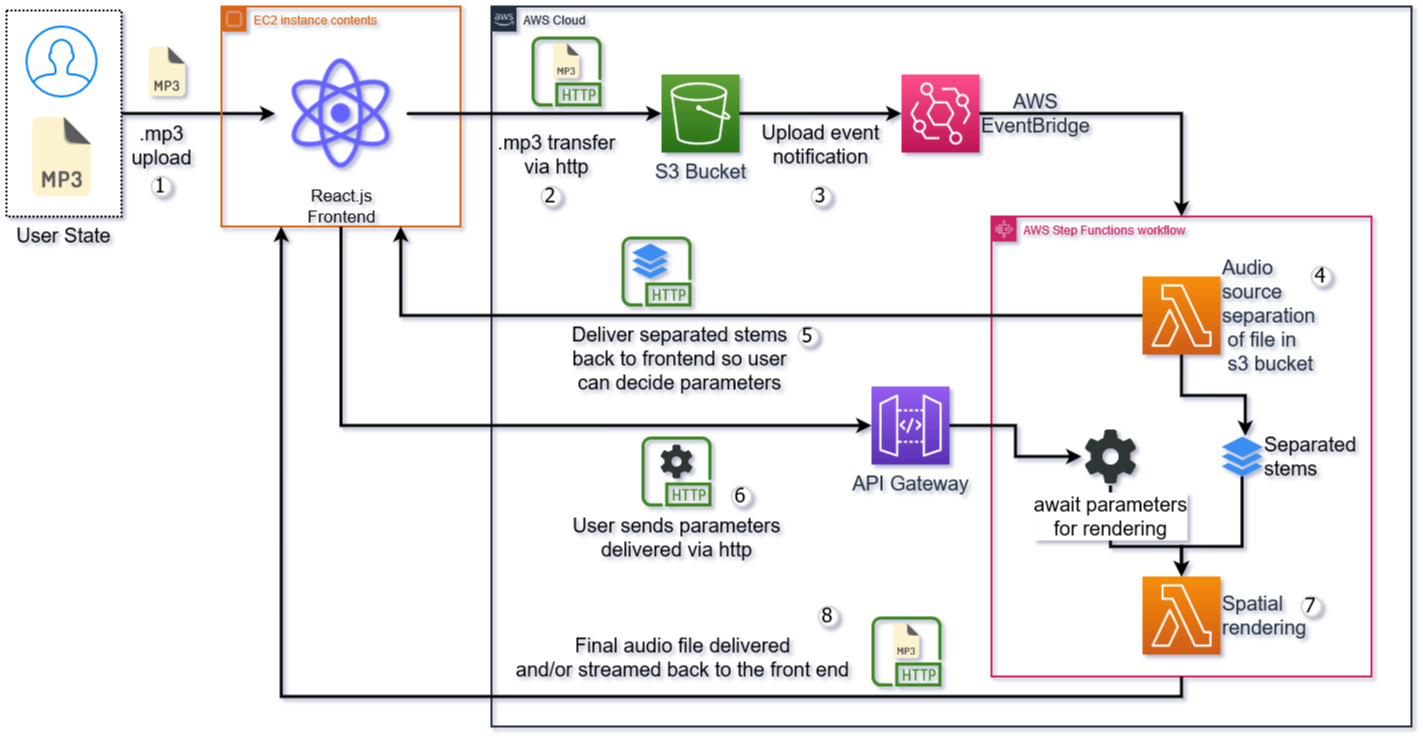
\includegraphics[width=1\textwidth]{architecture_diagram}
    \caption{Proposed architecture diagram}
    \label{fig:proposed_architecture}
    \centering
\end{figure}

Most of the tech stack has been detailed in Figure~\ref{fig:proposed_architecture}: a list of the technologies that are most likely to be utilised in the production of the final system are as follows:

\begin{enumerate}
    \item React.js frontend written in TypeScript
    \item Node.js frontend runtime
    \item Various AWS applications, including:
    \begin{itemize}
        \item \gls{ec2} to host the frontend application
        \item \gls{s3} bucket to store uploaded audio files and trigger upload events to begin the conversion process
        \item \gls{aws} EventBridge to process generated events
        \item \gls{aws} StepFunctions in order to schedule the audio conversion process
        \item \gls{aws} \gls{api} Gateway to receive parameters sent from the frontend via HTTP
    \end{itemize}
    \item WebRTC for audio streaming back to the user
    \item GitHub for version control and documentation
    \item LaTeX for documentation typesetting
    \item ClickUp software for project management
    \item Playwright for automated testing
\end{enumerate}

However, still some technologies that have yet to be decided on.\ A significant part of the research section of this project will be the determination of the audio source separation and spatial audio rendering engines that are to be used in the system.\ Some candidates for each have already been explored:

\begin{enumerate}
    \item Audio source separation:
    \begin{itemize}
        \item Spleeter by Deezer (Python)
        \item Open-Unmix
    \end{itemize}
    \item Spatial Audio Rendering:
    \begin{itemize}
        \item 3D TuneIn
        \item Resonance Audio
        \item LabSound
    \end{itemize}
\end{enumerate}

This list is expected to develop as the project progresses and new opportunities for iteration or refinement arise.

\section{Background Materials}\label{sec:background-materials}

Due to the multi-disciplinary nature of this project, the academic materials intended to be referenced may be split up into several sections.

\subsection{Audio Spatialisation}\label{subsec:audio-spatialisation}
Any discussion of audio spatialisation and human sound localisation must begin with ``Spatial Hearing'', a seminal book authored by~\cite{blauert_spatial_hearing}.\ It contains an authoritative exploration into how humans perceive sound in three-dimensional space.\ Such is the influence of the book that it is frequently cited in papers relating to some of the most modern methods of audio spatialisation~\citep{3d_tune_in}.\ As such, it is a must-read when preparing the literature review for this project.

Another early publication that is considered to be significant in this space is ``Periphony: With-Height Sound Reproduction''~\cite{gerzon_periphony}.\ This article details how periphonics may be captured achieved through the use of multi-channel recording.\ However, this project is concerned with the spatialisation of audio through the use of~\glspl{hrtf} and further literature will be concerned with virtual ambisonics where spatialised sound sources are rendered with convolution based on fixed~\glspl{hrtf}~\citep{noisternig_ambisonic}.

\subsection{Cloud Architecture}\label{subsec:cloud-architecture}

The benefits of cloud computing have been widely researched in the literature~\citep{cc_overview}.\ Since this project seeks to apply these benefits to the act of audio processing, the review will target any research done on the most efficient way to host compute-heavy applications like source separation and spatial rendering which can lead to some performance issues when not accounted for in the architecture design~\citep{cc_challenges}.

\subsection{Web Audio}\label{subsec:web-audio}

One of the main challenges facing the project relates to how the rendered audio will be delivered back to the user.\ For the~\gls{mvp} the system needs to simply output an audio file, however to improve the~\gls{ux} the frontend interface will ideally allow the user to listen to the audio through a web audio~\gls{api}~\citep{mdn_audio_api,w3c_audio_api}.

As a stretch-goal for the project, the system will be able to deliver the audio to the user through streaming.\ WebRTC, in combination with the paradigm of software-defined networking offered by~\gls{aws}, could be a powerful avenue to explore when it comes to delivering streamed audio over the internet~\citep{webrtc}.

\section{Project Plan}\label{sec:project-plan}

The project plan for this project will be structured out a discrete set of tasks.\ The ClickUp software allows for projects to be managed through a series of lists and tasks.\ These tasks form the backbone of the project and will have a completion date assigned to them.\ These times have then been plotted out on a Gantt chart as you can see in Figure~\ref{fig:project_plan_1}.\ Phase 1 of the project has been filled out with a greater amount of detail, listing the tasks needed in order to produce the materials needed for the interim report.\ Meanwhile, the implementation details in phase 2 (Figure~\ref{fig:project_plan_2})are more sparse since they will be further informed by the outcomes of the the first phase of development.

\begin{sidewaysfigure}[ht]
    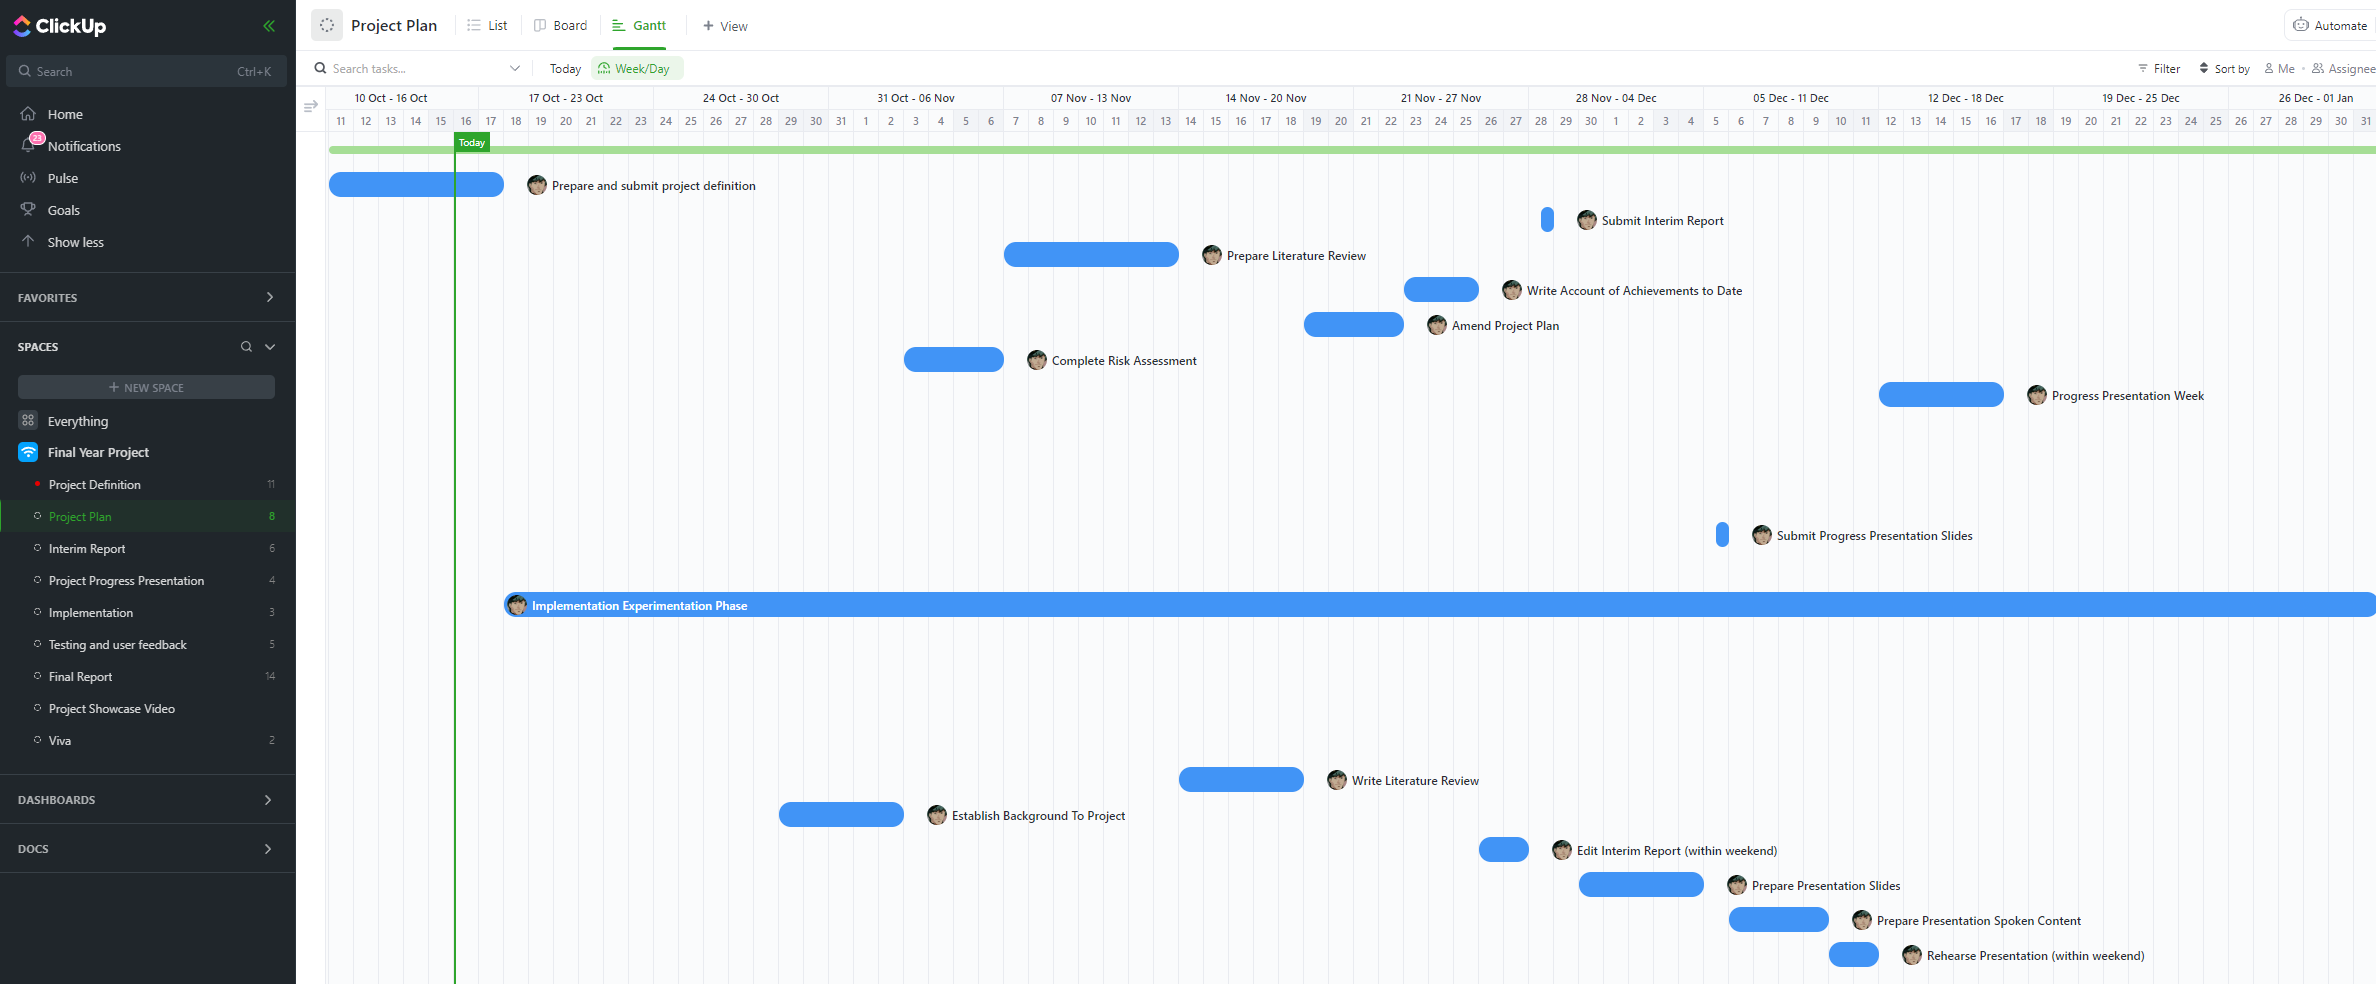
\includegraphics[width=1.1\textwidth]{project-plan-phase-1}
    \caption{Gantt chart hosted in ClickUp showing phase 1 of the project}
    \label{fig:project_plan_1}
\end{sidewaysfigure}

\begin{sidewaysfigure}[ht]
    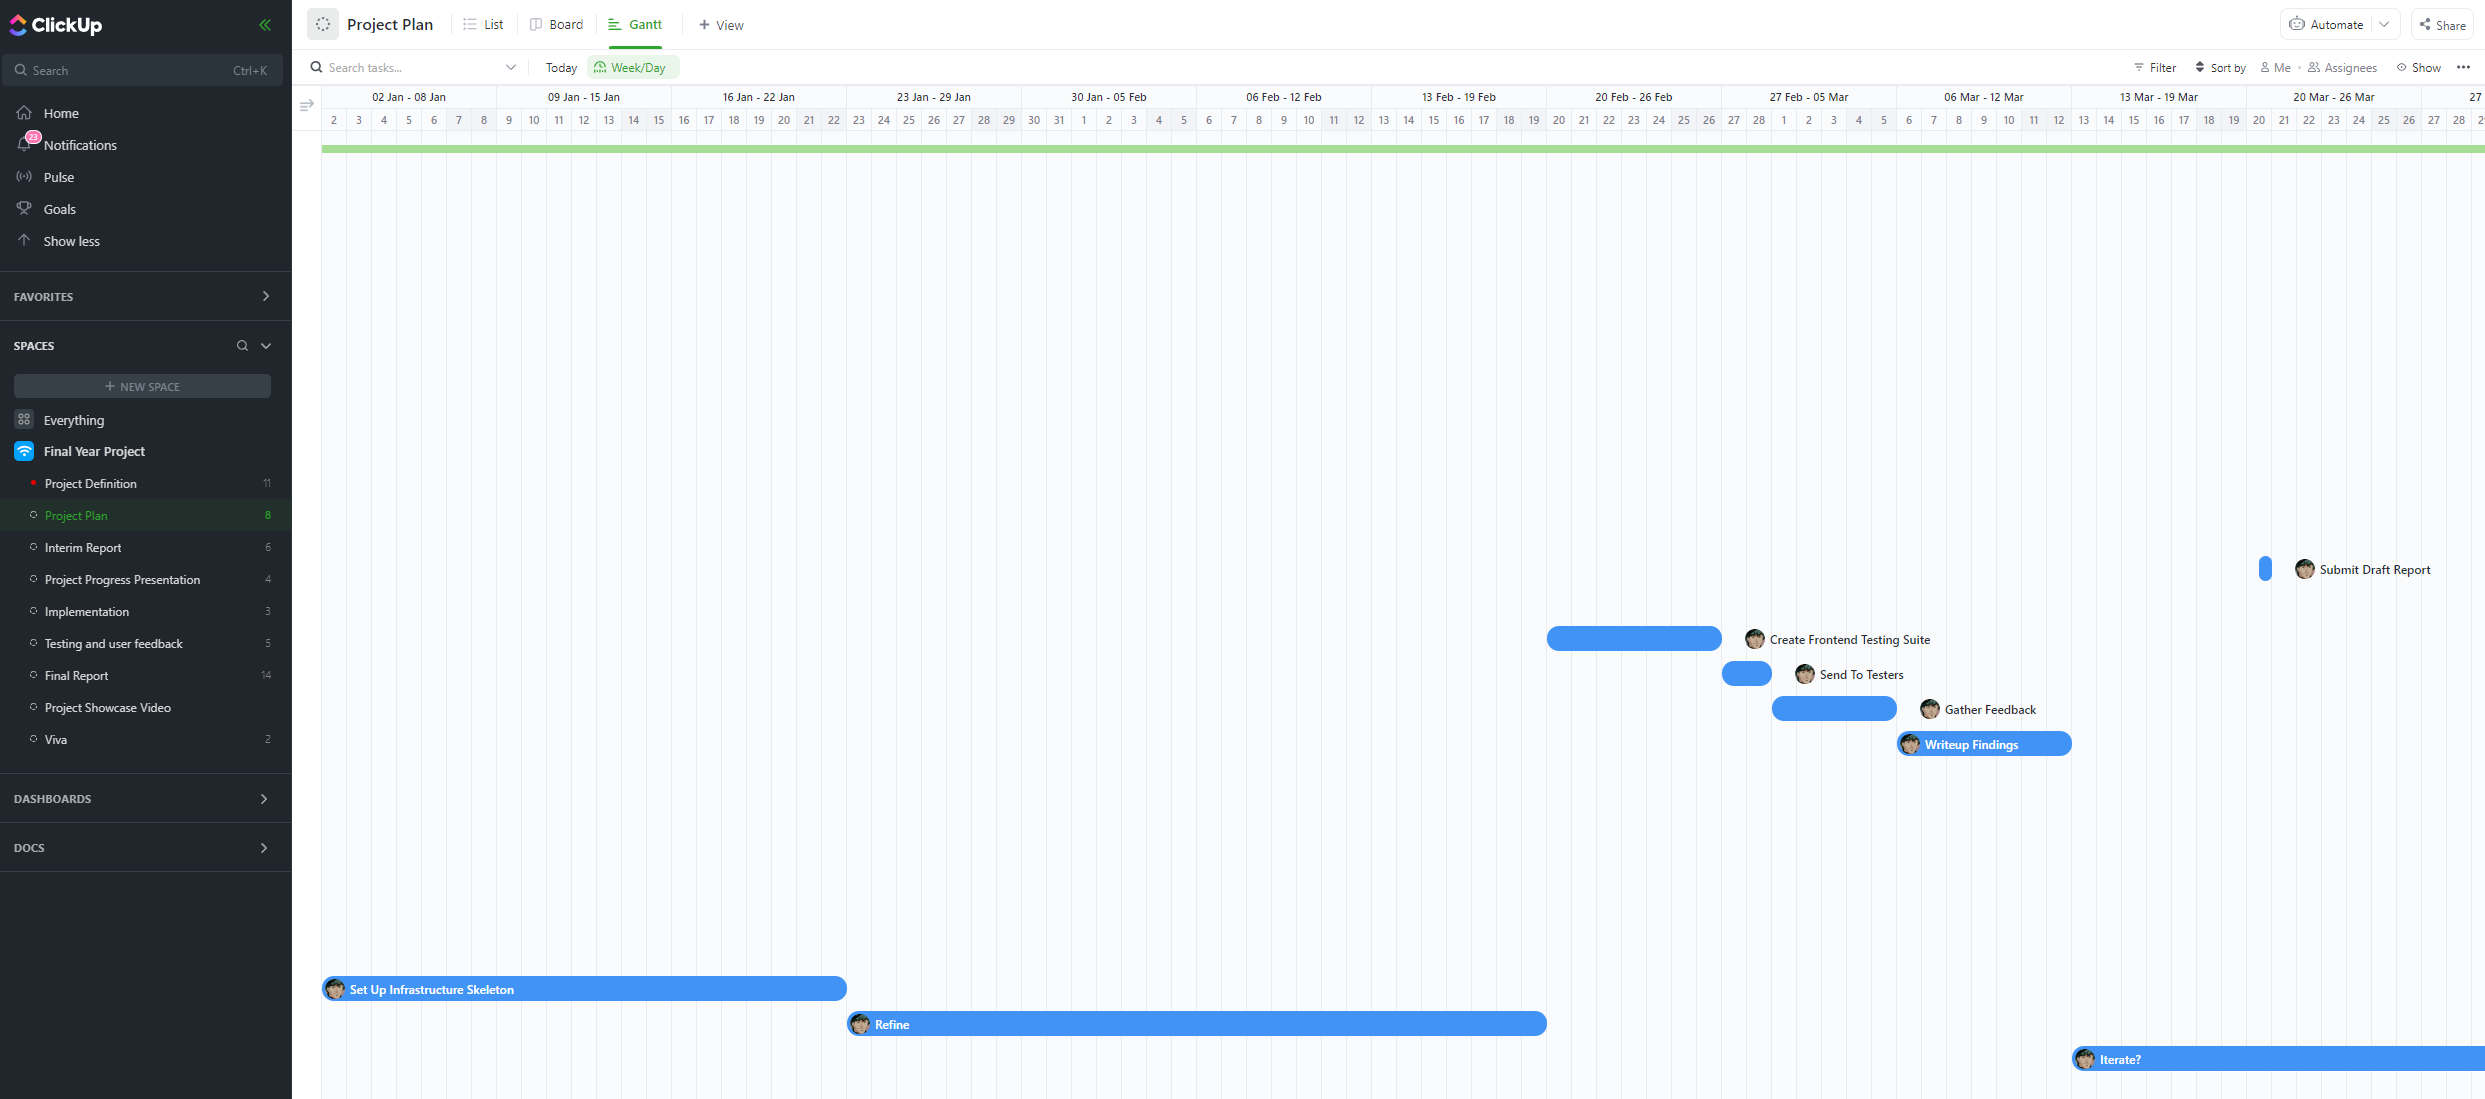
\includegraphics[width=1.1\textwidth]{project-plan-phase-2}
    \caption{Gantt chart hosted in ClickUp showing phase 2 of the project}
    \label{fig:project_plan_2}
\end{sidewaysfigure}

\bibliographystyle{agsm}
\bibliography{project-definition}

\printglossaries

\end{document}

